\documentclass[tikz,border=2pt]{standalone}
\usepackage{amsmath,amssymb}
\usepackage{tikz}

\begin{document}
% At least K = 2 of N = 4 inequalities must hold: each gets a relaxation switch y_i, and at
% most N - K = 2 switches may be on.
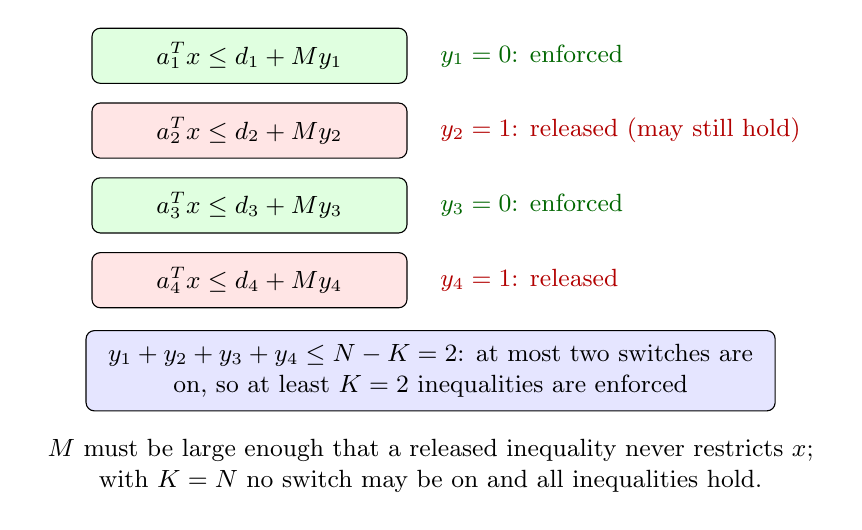
\begin{tikzpicture}[every node/.style={font=\small}, row/.style={draw, rounded corners=3pt, minimum width=4.0cm, minimum height=7mm, inner sep=4pt}]
	\node[row, fill=green!12] (r1) at (0,0) {$a_1^Tx\le d_1+My_1$};
	\node[row, fill=red!10] (r2) at (0,-0.95) {$a_2^Tx\le d_2+My_2$};
	\node[row, fill=green!12] (r3) at (0,-1.9) {$a_3^Tx\le d_3+My_3$};
	\node[row, fill=red!10] (r4) at (0,-2.85) {$a_4^Tx\le d_4+My_4$};
	\node[green!40!black, anchor=west] at (2.3,0) {$y_1=0$: enforced};
	\node[red!70!black, anchor=west] at (2.3,-0.95) {$y_2=1$: released (may still hold)};
	\node[green!40!black, anchor=west] at (2.3,-1.9) {$y_3=0$: enforced};
	\node[red!70!black, anchor=west] at (2.3,-2.85) {$y_4=1$: released};
	\node[draw, rounded corners=3pt, fill=blue!10, inner sep=5pt, text width=8.4cm, align=flush center] at (2.3,-4.0) {$y_1+y_2+y_3+y_4\le N-K=2$: at most two switches are on, so at least $K=2$ inequalities are enforced};
	\node[anchor=north, align=flush center, text width=10cm] at (2.3,-4.75) {$M$ must be large enough that a released inequality never restricts $x$; with $K=N$ no switch may be on and all inequalities hold.};
\end{tikzpicture}
\end{document}
